\section{Linear algebra}

In the previous section on general algebra we dealt with vector spaces (subspaces, linear independence, bases) and inner product spaces (norms, orthogonality). 
Here we'll mostly deal with the inner-product space of vectors and occasionally with the vector-space of matrices (but really, almost exclusively with the former ... ).




\subsection{Spaces}

We'll work a lot with a few vector-spaces and transfromations from and to those spaces. 

\begin{definition}
    Let $W$ be a space. Then $V \subseteq W$ is a subspace, if: 
    \begin{itemize}
        \item $\forall v_1, v_2 \in V: v_1 + v_2 \in W$
        \item $\forall v \in V: \forall r \in R: rv \in V$
    \end{itemize}
\end{definition}
    

\begin{definition}[Nullspace]
     $\nullspace{A}$ is the nullspace of $A$. It is defined as $\nullspace{A} = \{ x | Ax = 0 \}$
\end{definition}

\begin{definition}[Columnspace]
     $\collspace{A}$ is the collumnspace of $A$. It is defined as $\collspace{A} = \{ y | Ax = y \}$
\end{definition}

\begin{definition}[Rowspace]
     $\rowspace{A}$ is the rowspace of $A$. It is defined as $\rowspace{A} = \{ y | A^Tx = y \}$
\end{definition}

\begin{definition}[Rank]
     $r_A$ is the rank of $A$. It is defined as the dimension of $\collspace{A}$, $\dimension{\collspace{A}}$
\end{definition}

\begin{definition}[Nullity]
    $n_A$ is the nullity of $A$. It is defined as the dimension of $\nullspace{A}$, $\dimension{\nullspace{A}}$
\end{definition}


\paragraph{rops and cops as matrix multiplication} ...
$$ \rops(A) = \rops(I) A = R A$$
$$ \cops(A) = A \cops(I) = A C$$

\paragraph{rops don't change \nullspace{A}}
Row- and column-operations (rops and cops) seem somewhat trivial at first and not worth any proof writing efforts. However, many theorems of linear algebra are much easier proved if we first reduce the matrices to their RRLE (reduced row linear echelon) form.

\begin{theorem}
  Row-operations on $A$ don't change \nullspace{A}. 
\end{theorem}

\begin{proof}
    \subprf {Let $A' = \rops(A) = RA$} {\nullspace{A} = \nullspace{A'}} {
        \subprf {Let $x_0: Ax_0 = 0$} {$\exists y_0: A'y_0 = 0$} {
            \subprf {Try $y_0 = x_0$} {$A'y_0 = 0$} {
                $RAy_0 = 0$
            }
        } \\
        \subprf {Let $y_0: A'y_0 = 0$} {$\exists x_0: Ax_0 = 0$} {
            This is equivalent to stating that $\exists x_0: R^{-1} A' x_0 = 0$ \\
            \subprf {Try $x_0 = y_0$} {$R^{-1} A' x_0 = 0$} {
                $R^{-1} A' x_0 = 0$
            }
            
        }
    } 
\end{proof}

Therefore, when searching for the special solutions to a problem $Ab = 0$, we can use Gauss-Elemination and RREF without any problems.

\paragraph{cops don't change C(A)} ...

\paragraph{rops don't change C(A) if A is invertible }...

We can now print an overview of the different spaces that are associated with a matrix $A$ of dimension $m \cdot n$ and rank $r$.

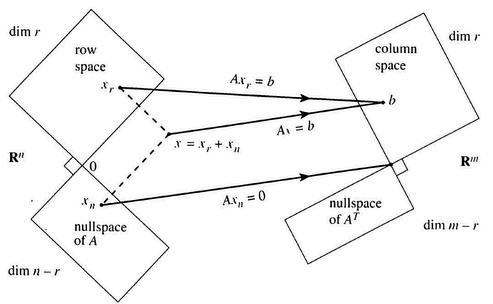
\includegraphics[width=0.7\linewidth]{images/four_spaces.png}

The rowspace of $A$ can be visualized using the line-intersection view of matrix-equations: it contains all the points that lie in the intersection of all the lines that make up the matrix. The columspace of A can be visulaized using the vector-image of A: it contains all the points that are spanned by A. 
Notice how we included the previous theorem: any combination $x$ of a particular sollution $x_r$ and any vector in the nullspace $x_n$ is also a solution.


We should look in more detail at this graphic. Note, for example, that \nullspace{A} and \collspace{A^T} seem to be orthogonal. Indeed:
\begin{theorem}
    [$\forall v \in \nullspace{A}, w \in \collspace{A^T}: v \orth w$]
\end{theorem}
\begin{proof}
    \begin{equation}
        \begin{aligned}
            w^T v &= 0  & \text{ with } \thereis u: \mtrx{A}^T u = w \\
            u^T \mtrx{A} v &= 0 & \text{ with } \mtrx{A}v = 0 \\
            u^T 0 &= 0 & \text{ which is trivially true.}
        \end{aligned}
    \end{equation}
    Thus, \nullspace{A} and \collspace{A^T} only intersect in $\vec{0}$.
\end{proof}

However, note that $\reals^n \geq \nullspace{A} \union \collspace{A^T}$. As an example, consider $\mtrx{A} = \begin{bmatrix}
    1 & 0 \\
    0 & 0
\end{bmatrix}$. We get $\nullspace{A} = \begin{bmatrix}
    0 \\ x
\end{bmatrix}$ and $\collspace{A^T} = \begin{bmatrix}
    x \\ 0
\end{bmatrix}$. Now consider $\vec{v} = \begin{bmatrix}
    1 \\ 1
\end{bmatrix}$, which is neither in \nullspace{A} nor in \collspace{A^T}. As illustration, look at fig. \ref{nullspace_rowspace_lowrank}.

\begin{figure}[H] \label{nullspace_rowspace_lowrank}
    \caption{When $A$ is not full rank, there are infinitely many vectors $v$ that are neither in \rowspace{A} nor in \nullspace{A}. When it comes to spatial dimensions, $1 + 1 \neq 2$!}
    \centering
    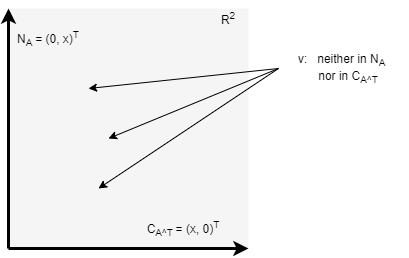
\includegraphics[width=0.5\linewidth]{images/nullspace_rowspace_lowrank.png}
\end{figure}





\subsection{Change of basis}\label{changeOfBasis}

Let $V$ be a vector space. Let $0$ be the canonical basis for that vector space. Let $A = \{\vec{a}_1, ..., \vec{a}_N \}$ and $B = \{\vec{b}_1, ..., \vec{b}_N\}$ be two other basis for that vectorspace. Let $\mtrx{A}$ be the matrix $[\vec{a}_1  ...  \vec{a}_N]$ and $\mtrx{B} = [\vec{b}_1 ... \vec{b}_N]$

Every vector $\vec{v}$ can be expressed as a linear sum of the basisvectors in $A$, that is $\vec{v} = \sum_n \alpha_n \vec{a}_n$. That same thing in matrix notation: $\vec{v} = \mtrx{A}(\vec{v})_A$, where $(\vec{v})_A$ is the coordinates $\alpha$ of $\vec{v}$ with respect to the basis $A$. Correspondingly, for $B$ we have $\vec{v} = \sum_n \beta_n \vec{b}_n = \mtrx{B}(\vec{v})_B$.

Note that within $A$ and $B$, we express the basevectors with respect to the canonical basis $0$, that is, we should really write $\mtrx{A} = [(\vec{a}_1)_0  ...  (\vec{a}_N)_0]$. Note also that $[(\vec{a}_1)_A  ...  (\vec{a}_N)_A] = \mtrx{I}$, the identity matrix. 

We can use this to obtain a simple formula for the change of basis. 
$$ \vec{v} = \mtrx{A} (\vec{v})_A $$
$$ \vec{v} = \mtrx{B} (\vec{v})_B $$
$$ (\vec{v})_B = \mtrx{B}^{-1} \mtrx{A} (\vec{v})_A $$

But inverses are notoriously hard to calculate. Fortunately, there is another approach. Call $\mtrx{T}_{BA} = [(\vec{a}_1)_B ... (\vec{a}_N)_B]$ the \emph{transition matrix}. We can prove that $\mtrx{B}^{-1} \mtrx{A} = \mtrx{T}_{BA}$:

\begin{equation}
\begin{aligned}
\mtrx{B}^{-1} \mtrx{A} (\vec{v})_A &= \mtrx{T}_{BA}  (\vec{v})_A \\
                                   &= \sum_n (v_n)_A (\vec{a}_n)_B \\
                                   &= \sum_n (v_n)_A \mtrx{B}^{-1} \mtrx{A} (\vec{a}_n)_A \\
                                   &= \mtrx{B}^{-1} \mtrx{A} \sum_n (v_n)_A (\vec{a}_n)_A \\
                                   &= \mtrx{B}^{-1} \mtrx{A} \text{  } \mtrx{I} (\vec{v})_A \\
                    (\vec{v})_A &=  (\vec{v})_A         
\end{aligned}
\end{equation}

Using $\mtrx{T}_{BA} = \mtrx{B}^{-1}\mtrx{A}$, a lot of statements are trivial to prove:
\begin{itemize}
    \item $\mtrx{T}_{BA} = \mtrx{T}_{AB}^{-1}$
    \item $\mtrx{T}_{CA} = \mtrx{T}_{CB} \mtrx{T}_{BA}$
\end{itemize}













\subsection{Linear transformations}

\begin{definition}
Let $U$ and $V$ be two vector spaces and $f:U \to V$. Then $f$ is a \emph{linear transform} if
\begin{itemize}
    \item $f$ preserves scalar multiplication: $f(\alpha \vec{u}) = \alpha f(\vec{u})$
    \item $f$ preserves vector addition: $f(\vec{u}_1 + \vec{u}_2) = f(\vec{u}_1) + f(\vec{u}_2)$
\end{itemize}
\end{definition}

There are a bunch of properties to linear transformations that can be useful to us. 

\begin{proof}[There is a unique linear transform from the basis of $U$ to any set of vectors in $V$ that we want.] In other words, any linear transform $f$ is completely deterimed by the matrix $[ f(\vec{b}_1) ... f(\vec{b}_N) ] = [\vec{v}_1 ... \vec{v}_N]$. That means if we dont know the transform, but we do know the results of the transform on a basis, then we can reconstruct the transform with certainty.  \\

    \subprf{Let $B = \{ \vec{b}_1, ..., \vec{b}_N \}$ be a basis for $U$. Let $\{ \vec{v}_1, ..., \vec{v}_N \}$ be any vectors in $V$ that we may chose. }
    { there is a unique function $f:U \to V$ such that $f(\vec{b}_i) = \vec{v}_i$ }{
    
        \subprf{Try $f(\vec{x}) = \mtrx{V} (\vec{x})_B$}
        {$f(\vec{b}_i) = \vec{v}_i$ and $f$ is a linear transform.}{
        
            \subprf{Part 1: }
            {$f(\vec{b}_i) = \vec{v}_i$}{
                
                $ f(\vec{b}_i) = \mtrx{V} (\vec{b}_i)_B = \mtrx{V} \vec{e}_i = \vec{v}_i $
                
            }
            
            \subprf{Part 2: }{$f$ is unique}{
                
                We could not have obtained any other form of $f$ than $f(\vec{x}) = \mtrx{V} (\vec{x})_B$. This is because for \emph{any} linear transform from $U \to V$ we have: 
                
                $ f(\vec{x}) = f(\mtrx{B}(\vec{x})_B) = f(\sum_n (x_n)_B \vec{b}_n) = \sum_n (x_n)_B f(\vec{b}_n)  $
                
                Using the result from part 1, this cannot be any other function than: 
                
                $ \sum_n (x_n)_B f(\vec{b}_n) = \sum_n (x_n)_B \vec{v}_n = \mtrx{V} (\vec{x})_B $ 
                
            }
            
            \subprf{Part 3: }
            {$f$ is a linear tansform}{
            
            }
        }
    }
\end{proof}

A whole bunch of other properties are now easily proved. Let $f$ and $g$ be linear transforms from $U$ to $V$. The following are also linear transforms: 
\begin{itemize}
    \item $\alpha f$
    \item $f + g$
    \item $f^{-1}$ ( if it exists )
    \item $fg$ ( here $g: V \to W$ )
\end{itemize}

Let $f: U \to V$ be a linear transform. Then the following are equivalent: 
\begin{itemize}
    \item If $f(\vec{u}) = \vec{0}$, then $\vec{u} = \vec{0}$
    \item $f$ is one-to-one
    \item $f$ maps linearly independent vectors to linearly independent vectors. 
\end{itemize}


Prove that a transform can be split up into mulitple transforms on the basis vectors. 
As an examle, consider the case of a rotation. A diagonal rotation can be reproduced by a rotation first around one, then around another axis. 


\paragraph{A linear transformation can also be a change of basis} when it is on a vectorspace and invertible.














\subsection{Linear independence}


\begin{definition}
    $B$ is linearly independent if $\forall b \in B: b \neq \sum r_n b_n$, with $b_n \in B/b$. 
\end{definition}

\begin{theorem} \label{lin_indep_if_no_bx0}
  A better definition could be stated as such: $B$ is linearly independent, if the only solution to $Bx = 0$ is the zero-vector.
\end{theorem}

\begin{proof}
    \subprf{Suppose $\forall \vec{b} \in \mtrx{B}: \vec{b} \neq \sum_{B/b} \alpha_i \vec{b}_i$}{$\mtrx{B}\vec{x} = \vec{0} \then \vec{x} = \vec{0}$}{
        \subprf{Suppose $\mtrx{B} \vec{x} = \vec{0}$}{$\vec{x} = \vec{0}$}{
            \subprf{By contradiction. Assume $\vec{x} \neq \vec{0}$}{there is a contradiction.}{
                We have $\mtrx{B}\vec{x} = \vec{0}$ \\
                Consider the vector $\vec{b}_3$. \\
                Thus: $\sum_{B/b_3} x_i \vec{b}_i = -x_3 \vec{b}_3$ \\
                Or: $\sum_{B/b_3} \frac{- x_i}{x_3} \vec{b}_i = -x_3 \vec{b}_3$ \\
                This contradicts the statement that $\forall \vec{b} \in \mtrx{B}: \vec{b} \neq \sum_{B/b} \alpha_i \vec{b}_i$
            }
        }
    }
    \subprf{Suppose $\mtrx{B}\vec{x} = \vec{0} \then \vec{x} = \vec{0}$}{$\forall \vec{b} \in \mtrx{B}: \vec{b} \neq \sum_{B/b} \alpha_i \vec{b}_i$}{
        \subprf{Let $\vec{b_0} \in \mtrx{B}$}{$\vec{b}_0 \neq \sum_{B/b_0} \alpha_i \vec{b}_i$}{
            \subprf{By contradiction. Assume $\vec{b}_0 = \sum_{B/b_0} \alpha_i \vec{b}_i$}{there is a contradiction.}{
                Since $\vec{b}_0 = \sum_{B/b_0} \alpha_i \vec{b}_i$ \\
                we get $\vec{0} = \sum_B \alpha_i \vec{b}_i$, where $\alpha_0 = -1$ \\
                In matrix notation: $\vec{0} = \mtrx{B} \vec{\alpha}$, with a non-zero $\vec{\alpha}$. \\
                This contradicts our assumption that $\mtrx{B}\vec{x} = \vec{0} \then \vec{x} = \vec{0}$
            }
        }
    }
\end{proof}

\begin{definition}
    Let $V$ be a subspace. $B \subseteq V$ is a basis for $V$ if $B$ is linearly independent and $\forall v \in V: v = \sum r_n b_n$, with $b_n \in B$
\end{definition}










\subsection{Determinant}

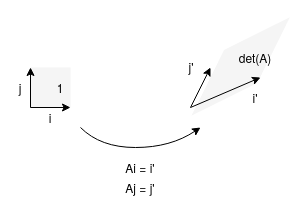
\includegraphics[width=0.4\linewidth]{images/determinant.png}


\paragraph{Definition} Consider a $2 \times 2$ matrix $\mtrx{A}$ 
$$
\mtrx{A} = 
\begin{bmatrix}
    a_{11} & a_{12} \\
    a_{21} & a_{22}
\end{bmatrix}
$$
$\det{\mtrx{A}}$ is defined as $a_{11}a_{22} - a_{12}a_{21}$. The definitions for higher order matrix-determinants are similar, but so extremely tedious that we just ignore them here. 


\begin{theorem}  \label{det_0}
    Let $ \mtrx{A} \vec{x} = 0 $ and $ \vec{x} \neq \vec{0}$. Then it must hold that $\det{\mtrx{A}} = 0$.
    In fact, this holds in two directions:

    $$ \thereis \vec{x} \neq \vec{0}: \mtrx{A} \vec{x} = 0  \iff \det{\mtrx{A}} = 0 $$
\end{theorem}
\begin{proof}
    We can prove this making use of theorem \ref{lin_indep_if_no_bx0}. From the given it follows that $\mtrx{A}$ is linearly dependent. 
    Thus $\thereis \vec{a} \in \mtrx{A}: \vec{a} = \sum_{A/a} \alpha_i \vec{a}_i$. In the case of a $2 \times 2$ matrix this expression becomes very simple: $\vec{a}_1 = \alpha \vec{a}_2$. 
    Breaking $\vec{a}_1$ into its components
    \begin{itemize}
        \item $a_{11} = \alpha a_{12}$
        \item $a_{21} = \alpha a_{22}$
    \end{itemize}
    Putting this into the definition of a determinant we get:
    \begin{equation}
        \begin{aligned}
            \det{\mtrx{A}}  &= a_{11}a_{22} - a_{12}a_{21} \\
                            &= \alpha a_{12} a_{22} - \alpha a_{12} a_{22} \\
                            &= 0
        \end{aligned}
    \end{equation}
    For higher order matrices, the proof follows from induction or something like that.
\end{proof}



\paragraph{Interpretation} The size of the determinant can be seen as the scaling-factor of the transformation described by the matrix $A$.
It is also a measure of how much linearly independent the rows/cols of $A$ are. The size of the determinant equals the size of the (hyper-)parallelogram spanned by the columns. If two vectors are almost linearly dependent, they will be almost parallel, leading to a very small area of the parallelogram. So if you have a small determinant, your columns are almost dependent. If you have a large one, your columns are very orthogonal. 
If your determinant is zero, that means that your matrix $A$ is a transformation $Ax$ that squishes (at least) one of the dimensions of $x$ into nothing.


\paragraph{Properties}
\begin{itemize}
    \item $\det{\mtrx{A} \mtrx{B}} = \det{\mtrx{A}}\det{\mtrx{B}}$
    \item $\det{\mtrx{A} + \mtrx{B}} \neq \det{\mtrx{A}} + \det{\mtrx{B}}$
    \item $\det{\mtrx{A}} = \prod{\lambda_i}$ (see eivenvalues, later)
\end{itemize}









\subsection{Rank nullity Theorem}


\begin{theorem}
    $ \nullspace{A} = \{ 0 \} \then \det{A} \neq 0 $
\end{theorem}
\begin{proof}
    This is almost self-proving. 
    $\nullspace{A} = \{ 0 \}$ is equivalent to writing $\mtrx{A} \vec{x} = \vec{0} \then \vec{x} = \vec{0}$.
    By theorem \ref{lin_indep_if_no_bx0} this means that $\mtrx{A}$ is linearly independent.
    And by theorem \ref{det_0} this means that $ \det{A} \neq 0 $.
\end{proof}


\begin{theorem}
    Let $A: X \to Y$. Then:
    $$ \nullspace{A} = \{ 0 \} \then \collspace{A} = Y $$
\end{theorem}

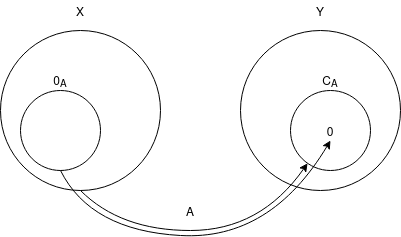
\includegraphics[width=0.4\linewidth]{images/A_from_X_to_Y.png}

\begin{theorem}
    Rank nullity: this is a fundamental theorem of linear algebra.
    Let $A$ be of dimension $r \times c$ and full rank.
    Then: 
    $$ r_A + n_A = c $$
\end{theorem}


\begin{theorem}
    $$ r_A = \dimension{\collspace{A}} = \dimension{\rowspace{A}} $$
\end{theorem}

\begin{theorem}
    $$ A:basis_{\collspace{A}} \then r_A = n $$
\end{theorem}






\subsection{Special matrices}

\paragraph{Symmetric matrices} are simple but very useful.
\begin{definition}
    [A matrix $\mtrx{A}$ is symmetric] iff $\mtrx{A} = \mtrx{A}^T$
\end{definition}


\paragraph{Positive (semi-)definite matrix} are a special case of symmetric matrices.
\begin{definition}
    [$\mtrx{A}: \PSD \iff \mtrx{A}: \symm \land \forall z: z^T \mtrx{A} z \geq 0$]
    From the first condition, $\mtrx{A}: \symm$, it follows that the eigenvectors are orthogonal (see eq. \ref{symm_then_orth}), 
    from the second one, $\forall z: z^T \mtrx{A} z \geq 0$, it follows that the eigenvalues are all greater or equal than $0$ (see eq. \dots).
\end{definition}


\paragraph{Gram matrices} appear often in important theorems. They turn out to be PSD.
\begin{definition}
    [A Gram matrix] is a matrix $\mtrx{A} = \mtrx{B}^T \mtrx{B}$
\end{definition}

\begin{theorem}
    [$\rank{A} = \rank{A^T A}$]
\end{theorem}

\begin{theorem}
    [$A^T A: \PSD$]
\end{theorem}


\paragraph{Orthogonal matrices} make tons of calculations simpler.
\begin{definition}[A matrix $\mtrx{A}$ is orthogonal] iff $\forall x_1, x_2 \in \mtrx{A}, x_1 \neq x_2: x_1 \orth x_2$
\end{definition}

\begin{theorem}
    [If $A$ is orthogonal, than $A^{-1} = A^T$.]
    This is trivially proven. By the definition of orthogonality we have $\mtrx{A}^T \mtrx{A} = \mtrx{I}$
\end{theorem}








\subsection{Eigenvalues and eigenvectors}

\begin{equation}
    \begin{aligned}
        A e &= \lambda e \\
        ( A - \lambda I ) e &= 0 \\
        \det{A - \lambda I} &= 0 \text{ using theorem \ref{det_0}}
    \end{aligned}
\end{equation}

Any \emph{square} matrix can be eigenvector (aka. spectrally) decomposed: $\mtrx{A} = \mtrx{E} \mtrx{\Lambda}\mtrx{E}^{-1}$.



Once at a sprint-discussion I wondered why principal components (see about those later) were all orthogonal. Here's the proof why. (Note that the proof only holds for symmetric matrices - which, in PCA, $C_A$ is indeed symmetric.)
\begin{theorem} \label{symm_then_orth}
    $\mtrx{A}: \symm \then \mtrx{E}_A: \orth$

    For any matrix $A$, symmetric or not, and for any vectors $x$ and $y$, eigenvectors or not, it holds:
    $\forall A, \forall x, y: <Ax, y> = <x, A^Ty>$
    This is true because 
    \begin{equation}
        \begin{aligned}
            <x, y>      &= x^T y \\
            <Ax, y>     &= (Ax)^T y \\
                        &= x^T A^T y \\
            <x, A^Ty>   &= x^T A^T y
        \end{aligned}
    \end{equation}
    Then we can use that finding as follows for $\mtrx{A}: \symm$ and $x, y \in \mtrx{E}_A$:
    \begin{equation}
        \begin{aligned}
                                                                & <Ax, y>           &= <x, A^Ty> \\
            \text{Since } A:\symm:                              & <Ax, y>           &= <x, Ay> \\
            \text{Since } x, y \text{ are eigenvalues of } A:   & <\lambda_x x, y>  &= <x, \lambda_y y> \\
                                                                & \lambda_x <x, y>  &= \lambda_y <x, y>
        \end{aligned}
    \end{equation}
    Thus, either $\lambda_x = \lambda_y$ or $x \orth y$ 
\end{theorem}

\begin{theorem}
    [As a corollary, the eigenvalue decomposition can be simplified]: $\mtrx{A}: \symm \then \mtrx{A} = \mtrx{X} \mtrx{\Lambda} \mtrx{X}^{-1} = \mtrx{X} \mtrx{\Lambda} \mtrx{X}^T$
\end{theorem}

\paragraph{Interpretation of eigenvalues}
\begin{itemize}
    \item $\lambda$ is complex: $\mtrx{A}$ contains a rotation
    \item $\lambda$ is negative: $\mtrx{A}$ contains some mirroring
    \item $\lambda$ is 0: $\det{\mtrx{A}} = 0$, i.e. $\mtrx{A}$ squishes a dimension
\end{itemize}




\subsection{Singular value decomposition}
Let $\mtrx{A}$ be of size $m \times n$. We will prove that also such non-square matrices can be decomposed, too, namely into:
\begin{equation}
    \mtrx{A} = \mtrx{U} \mtrx{\Sigma} \mtrx{V}^T
\end{equation}
where:
\begin{itemize}
    \item $\mtrx{U}$ and $\mtrx{V}$ are orthonormals of sizes $m \times m$ and $n \times n$, respectively
    \item $\mtrx{\Sigma}$ is a diagonal matrix of size $m \times n$
\end{itemize}
In other words: 
\begin{equation}
    \mtrx{A} \mtrx{V} = \mtrx{U} \mtrx{\Sigma}
\end{equation}
We'll find an orthonormal basis $\mtrx{V} \subset R_A$ which is transformed into an orthonormal basis $\mtrx{U} \subset C_A$.


We'll work with a practical example alongside the proof. Let $\mtrx{A} = \begin{bmatrix}
  2 & 0 \\
  0 & 1 \\
  0 & 2   
\end{bmatrix}$.

Consider $\mtrx{A}^T \mtrx{A}$. Contrary to $\mtrx{A}$, this is a psd matrix. It has eigenvectors $[\vec{e}_1, \vec{e}_2, ...] = \mtrx{E}_{A^TA} = \begin{bmatrix}
    1 & 0 \\
    0 & 1
\end{bmatrix}$ and eigenvalues 4 and 5.

Now consider the vector $\vec{y}_i = \mtrx{A} \vec{e}_i$. Multiplying both sides with $\lambda_i$ we observe that:
\begin{equation}
    \begin{aligned}
        \lambda_i \vec{y}_i &= \lambda_i \mtrx{A} \vec{e}_i \\
                            &= \mtrx{A} \lambda_i \vec{e}_i \\
                            &= \mtrx{A} \mtrx{A}^T \mtrx{A} \vec{e}_i \\
                            &= \mtrx{A} \mtrx{A}^T \vec{y}_i
    \end{aligned}
\end{equation}
In other words: $\vec{y}_i$ is an eigenvector of $\mtrx{A} \mtrx{A}^T$ with eigenvalue $\lambda_i$.

Indeed: $\mtrx{A} \mtrx{A}^T = \begin{bmatrix}
    4 & 0 & 0 \\
    0 & 1 & 2 \\
    0 & 2 & 4
\end{bmatrix}$ and $\mtrx{A} \mtrx{A}^T \myarray{0 \\ 1 \\ 2} = 5 \myarray{0 \\ 1 \\ 2}$.

A note on the size of $\vec{y}_i$: $|\vec{y}_i| = |\mtrx{A} \vec{e}_i| = \sqrt{|\mtrx{A}\vec{e}_i|^2} = \sqrt{\vec{e}_i^T \mtrx{A}^T \mtrx{A} \vec{e}_i} = \sqrt{\lambda_i} |\vec{e}_i|$.
If we want $\vec{y}_i$ to have normalized size we redefine it as $ \vec{y}_i = \frac{1}{\sqrt{\lambda_i}} \mtrx{A} \vec{e}_i $

Also, if $\lambda_i = 0$ then $\vec{y}_i = \vec{0}$.


Now, let $k = \rank{\mtrx{A}}$ and define the following new matrices:
\begin{equation}
    \begin{aligned}
        \hat{\mtrx{U}} &= [\vec{y}_i / \text{ where } \lambda_i = 0], \text{ size } m \times k  &= \begin{bmatrix}
                                                                                                        0 & 1 \\
                                                                                                        \frac{1}{\sqrt{5}} & 0 \\
                                                                                                        \frac{2}{\sqrt{5}} & 0
                                                                                                    \end{bmatrix}  \\
        \hat{\mtrx{V}} &= [\vec{e}_i / \text{ where } \lambda_i = 0], \text{ size } b \times k &= \begin{bmatrix}
                                                                                                        1 & 0 \\
                                                                                                        0 & 1
                                                                                                    \end{bmatrix}
    \end{aligned}
\end{equation}

Consider $\hat{\mtrx{U}}^T \mtrx{A} \hat{\mtrx{V}} \vec{b}_i$, where $\vec{b}_1 = \myarray{1 \\ 0}, \vec{b}_2 = \myarray{0 \\ 1}$:
\begin{equation}
    \begin{aligned}
        \hat{\mtrx{U}}^T \mtrx{A} \hat{\mtrx{V}} \vec{b}_i  &= \hat{\mtrx{U}}^T \mtrx{A} \vec{e}_i \\
                                                            &= \frac{1}{\lambda_i} \hat{\mtrx{U}}^T \mtrx{A} \lambda_i \vec{e}_i \\
                                                            &= \frac{1}{\lambda_i} \hat{\mtrx{U}}^T \mtrx{A} \mtrx{A}^T \mtrx{A} \vec{e}_i \\
                                                            &= \frac{1}{\lambda_i} \hat{\mtrx{U}}^T \mtrx{A} \mtrx{A}^T \vec{y}_i \sqrt{\lambda_i} \\
                                                            &= \frac{1}{\sqrt{\lambda_i}} \hat{\mtrx{U}}^T \mtrx{A} \mtrx{A}^T \vec{y}_i \\
                                                            &= \frac{1}{\sqrt{\lambda_i}} \hat{\mtrx{U}}^T \lambda_i \vec{y}_i \\
                                                            &= \sqrt{\lambda_i} \hat{\mtrx{U}}^T \vec{y}_i \text{, now, making use of } \hat{\mtrx{U}} \vec{b}_i = \vec{y}_i \\
                                                            &= \sqrt{\lambda_i} \vec{b}_i
    \end{aligned}
\end{equation}
Generally:
\begin{equation}
    \begin{aligned}
        \hat{\mtrx{U}}^T \mtrx{A} \hat{\mtrx{V}} \mtrx{I} &= \sqrt{\lambda_i} I \\
        \hat{\mtrx{U}}^T \mtrx{A} \hat{\mtrx{V}}   &= \mtrx{\Sigma}
    \end{aligned}
\end{equation}
where in our case $\mtrx{\Sigma} = \begin{bmatrix}
    0 & \sqrt{5} \\
    \sqrt{4} & 0 
\end{bmatrix}$

We'll now expand
\begin{itemize}
    \item $k \times m$ matrix $\hat{\mtrx{U}}$ to $m \times m$ matrix $\mtrx{U} = [\vec{y}_i]$, even where $\lambda_i = 0$
    \item $k \times n$ matrix $\hat{\mtrx{V}}$ to $n \times n$ matrix $\mtrx{V} = [\vec{e}_i]$, even where $\lambda_i = 0$
    \item $k \times k$ matrix $\mtrx{\Sigma}$ to $m \times n$ matrix $\mtrx{\Sigma} = \begin{cases}
        \text{if } i = j \land i < k: \sqrt{\lambda_i} \\
        \text{else } 0
    \end{cases}$
\end{itemize}
With that we obtain
\begin{equation}
    \mtrx{A} = \mtrx{U} \mtrx{\Sigma} \mtrx{V}^T
\end{equation}
In our example case we have 
$$
    \mtrx{\Sigma} = \begin{bmatrix}
        \sqrt{5} & 0 \\
        0        & 0 \\
        0        & \sqrt{4}
    \end{bmatrix}
$$




\paragraph{Example for a shear-matrix}: SVD means that any matrix-transformation can be rewritten as a rotation, scale and another rotation. Even a shear-matrix!
\begin{lstlisting}
M = [
    [1, .5],
    [0, 1]
]

U, S, VT = np.linalg.svd(M)

U @ (np.eye(2) * S) @ VT
\end{lstlisting}
SVD is often used for image compression, too. Just leave out some lower $\sigma_i$'s, then you can also leave out equally many columns / rows of $U$ and $V^T$, respectively.


\subsubsection{Principal component analysis}
Consider a $m \times n$ matrix $\mtrx{A}$. Let $\mtrx{X} = \mtrx{A} - \mtrx{\mu}$, the matrix with its mean subtracted.
Then we can express the covariance of $\mtrx{X}$ as $\mtrx{C}_X = \mtrx{X}^T \mtrx{X}$.

We want to find a transformation $\mtrx{P}$ such that $\mtrx{Y} = \mtrx{X} \mtrx{P}$ is uncorrelated. We'll prove that such a matrix does exist.
\begin{equation}
    \thereis \mtrx{P}: \mtrx{Y} = \mtrx{X} \mtrx{P} \land \mtrx{C}_Y: \text{diag}
\end{equation}

Try $\mtrx{P} = \mtrx{E}_{C_X}$. Then:
\begin{equation}
    \begin{aligned}
        \mtrx{C}_Y  &= \mtrx{Y}^T \mtrx{Y} \\
                    &= (\mtrx{X} \mtrx{P})^T \mtrx{X} \mtrx{P} \\
                    &= \mtrx{P}^T \mtrx{X}^T \mtrx{X} \mtrx{P} \\
                    &= \mtrx{P}^T C_\mtrx{X} \mtrx{P} \\
                    &= \mtrx{E}_{C_X}^T C_X \mtrx{E}_{C_X}
    \end{aligned}
\end{equation}
Thus $C_Y = \Lambda_{C_X}$, which is diagonal, as required.


Note: Sometimes we care not about $cov(n_1, n_2)$ but about $cov(m_1, m_2)$. Then we use: $C_X = \mtrx{X} \mtrx{X}^T$ and $\thereis \mtrx{P}: Y = \mtrx{P}\mtrx{X}$. Try $\mtrx{E}_{C_X}$

    










\subsection{Inverse}

If $A$ has dimensions $n \times n$, then the inverse $A^{-1}$ such that
$$ A A^{-1} = A^{-1} A = I $$
exists iff $det_A \neq 0$.

\paragraph{Nonsqare} matrices do not have an inverse, but they might have a right- or left-inverse.
Consider $C = A A^T$. This is a square matrix, so it might have an inverse:
$$ A A^T (A A^T)^{-1} = I $$
Calling $A^T (A A^T)^{-1} = A^{RI}$ the right inverse:
$$ A A^{RI} = I $$
For $C^{-1}$ to exist, we require $C$ to be full-rank, which means that $A$ must be full row rank. This  requires $r \leq c$, in other words, $A$ being a broad matrix.

\begin{proof}
If $A^{RI}$ exists, then $A^{LI}$ does not
\end{proof}

\begin{proof}
    $A^{RI}$ is not unique.
    Let $A$ be of dimension $r \times c$ and full rank, with $r < c$. By rank nullity we have
    $$ n_A = c - r > 0 $$
    That is, the nullspace is nonempty. Thus $\thereis x : Ax = 0$
    Now try $B' = B + x$
    We get 
    $$ AB' = AB + Ax = I + 0$$
\end{proof}


















\subsection{Applications}


\subsubsection{Systems of linear equations}
If there are more variables than equations, the system is underdetermined. If there are more eqations than variables, the system is overdetermined. A potentially solveable system is one where there are equally many variables as equations. But even then we must distinguish two cases. 

\paragraph{Solving well determined systems}
There are two cases: a system is either consistent or inconsistent. The follwing statements are all equivalent, meaning that any one of them is related to any other one in an if-and-only-if way. 

\begin{itemize}
    \item the system is consistent
    \item the matrix is invertible
    \item the determinant is nonzero
    \item there is exactly one sollution
\end{itemize}

We proof a few of those equivalences just for the hell of it. 

\begin{proof} There is exactly one solution if and only if the determinant is nonzero. \\
    \subprf{}{$|A| = 0 \iff \thereis ! \vec{x} : A \vec{x} = \vec{b} $}{
    
    }
\end{proof}

On the other hand, in the inconsistent case, the follwing statements are equivalent:

\begin{itemize}
    \item the system is inconsistent
    \item the matrix is singular (aka. noninvertible)
    \item the determinant equals zero
    \item one (or more) row (or column) is lineraly dependent of the others
\end{itemize}

\paragraph{Solving overdetermined systems: least squares}


\paragraph{Solving underdetermined systems: geometric bodies}
I like to think of underdetermined systems as (linear) geometric bodies, written in their parameterized form. A line in $\reals^3$ is described by a $3 \times 1$ matrix (or rather, it's column space), a plane in $\reals^3$ by a $3 \times 2$ matrix. However, it is important to note one distinction: geometric objects don't need to go through the origin, a matrix system however does. A line that does not go through the origin needs a base vector, like so: 

$$\vec{x} = \begin{bmatrix} \vec{d} \end{bmatrix} \begin{bmatrix} \alpha \end{bmatrix} + \vec{b}$$ 

A plane that does not go through the origin also needs a base vector $\vec{b}$, like so: 

$$\vec{x} = \begin{bmatrix} \vec{p}_1 && \vec{p}_2 \end{bmatrix} \begin{bmatrix} \alpha  \\ \beta \end{bmatrix} + \vec{b}  $$



Here is a problem that bothered me for a while: a line needs one parameter, a plane two. An ellipsoid, too, needs two parameters. Are there any linear geometric objects in $\reals^3$ that require more than three parameters? The answer is: no. Here is the proof. 

\begin{proof}
    For any $3 \times 4$ matrix, there is a $3 \times 3$ matrix that has the same column space, that is, that describes the same geometrical body. \\
    
    \subprf{}{$\forall A(3 \times 4) \thereis A'(3 \times 3): \collspace{A} = \collspace{A'}$}{

        \subprf{Let $A_0(3 \times4)$.}{$\thereis A': \collspace{A_0} = \collspace{A'}$}{
        
            We know from \ref{proofBaseSizeEqualsSpaceDimension} that $\thereis \vec{a}_0 \in A_0: \vec{a}_0:ld$. So Try $A' = A_0/\vec{a_0}$.
            
            Indeed, now $A_0$ and $A'$ both form a base of the same space. So they must have the same column space. 
        }    

    }
\end{proof}

However, there are \emph{non}linear objects in $\reals^3$ that require more than three parameters! Many curves in 3d require many parameters. \emph{But} those curves don't form a vector-space, while lines and planes do (as long as they go through the origin). 


\paragraph{Summary}
\begin{table}[ht]
\centering
\caption{Influence of rank on solutions}
\begin{tabular}{@{}llll@{}}
\toprule
                                                                                      & m \textless n                             & m = n & m \textgreater n                                 \\ \midrule
\rowcolor[HTML]{96FFFB} 
\cellcolor[HTML]{96FFFB}                                                              & n - m free variables                      &       &                                                  \\
\rowcolor[HTML]{96FFFB} 
\multirow{-2}{*}{\cellcolor[HTML]{96FFFB}r \textless m}                               & m – r conditions on $b \in \collspace{A}$ &       &                                                  \\
                                                                                      & 1 pivot per row                           &       &                                                  \\
                                                                                      & n – r = n – m free variables              &       &                                                  \\
\multirow{-3}{*}{\begin{tabular}[c]{@{}l@{}}r = m \\ (full row rank)\end{tabular}}    & 0 conditions on $b \in \collspace{A}$     &       & X                                                 \\
\rowcolor[HTML]{96FFFB} 
\cellcolor[HTML]{96FFFB}                                                              &                                           &       & m – r conditions on $b \in \collspace{A}$        \\
\rowcolor[HTML]{96FFFB} 
\multirow{-2}{*}{\cellcolor[HTML]{96FFFB}r \textless n}                               &                                           &       & n – r free variables                             \\
                                                                                      & X                                         &       & 1 pivot per column                               \\
                                                                                      &                                           &       & m – r = m – n conditions on $b \in \collspace{A}$ \\
\multirow{-3}{*}{\begin{tabular}[c]{@{}l@{}}r = n \\ (full column rank)\end{tabular}} &                                           &       & 0 free variables, thus $\nullspace{A} = \{0\}$     \\ \cmidrule(l){1-4} 
\end{tabular}
\end{table}




\paragraph {Ax = b reduces to A'x' = 0}

\begin{theorem}
  A problem of the form $Ax = b$ can be re-expressed as $A'x' = 0$, where $A' = [A, -b]$ 
\end{theorem}

\begin{proof}
    \subprf {} {$A x = b$ can be re-expressed as $A'x' = 0$} {
        $ A x = b $ \\
        $ A x -b = 0 $ \\
        $ A_1 x_1 + A_2 x_2 + ... -b = 0 $ \\
        Let $A' = [A, b]$ and $x_{n+1} = -1$. Then: \\
        $ A' x' = 0 $ \\
        Now we can use the nullspace of $A'$ to find the solutionspace of $A$. \\
        $ \nullspace{[A b]} = \{x' | [A b]x' = 0\} $ \\
        $ = \{x' | A x'_{1:m} = -b x'_{m+1}\} $ \\
        A subset of that nullspace equals the solutionset for $A x = b$: \\
        $ \nullspace{[A b]} \text{ where } [x'_{m+1} = -1] = \{x'| A x'_{1:m} = b \} $ 
    }   
\end{proof}


\paragraph{Solving Ax = b}

\begin{theorem}
  If we can only find any one particular solution $x_p$ such that $A x_p = b$, then we get the whole solutionspace as $\nullspace{A} + x_p$.
\end{theorem}

\begin{proof}
    \subprf{Let $x_p: A x_p = b$.}{$\solspace{A x = b} = \nullspace{A} + x_p$}{
        We'll make use of the fact that $\nullspace{A} + x_p = \{ x + x_p | A x = 0 \} = \{ x | A x = A x_p \}$ \\
        \subprf{Let $x_0 \in \nullspace{A} + x_p $.}{$x_0 \in \solspace{A x = b}$, i.o.w. $A x_0 = b$}{
            $ x_0 \in \nullspace{A} + x_p $ \\
            $ x_0 \in \{ x + x_p | A x = 0 \} $ \\
            $ x_0 \in \{ x | A (x - x_p) = 0 \} $ \\
            Thus $ A x_0 = A x_p $ \\
            Since $A x_p = b$, it must be that $ A x_0 = b $.
        }
        \subprf{Let $x_0 \in \solspace{A x = b}$.}{$x_0 \in \nullspace{A} + x_p$, i.o.w. $A x_0 = A x_p$}{
            Because $x_0 \in \solspace{A x = b}$, we have $A x_0 = b$. \\
            Also, it was given that $A x_p = b$.
        }
    }
\end{proof}





\subsubsection{Matrix factorisation}

\paragraph{Eigenvalue decomposition}
$$ A = V \Lambda V^{-1} $$

\paragraph{Singular value decomposition} is eigenvalue decomposition, generalized to non-square matrices.
$$ A = U \Sigma V^T $$

\paragraph{Nonnegative matrix factorisation}: Consider a dataset $A$, mapping people (rows) to properties (columns). You are looking for some hidden, small set of features, that groups of people have in common. 
In neural networks we can reconstruct images from a minimal amount of hidden features by funnelling the image through a very small hidden layer out to a large output layer. We can do the very same thing here!
$$ A = U V $$
Where $A$ has dimension $r \times c$, $U$ associates people with their hidden features/groups $r \times f$ and $V$ associates features/groups with the properties $f \times c$.
